\documentclass[11pt,a4paper]{article}
\usepackage[top=3cm, bottom=2cm, left=2cm, right=2cm]{geometry}
\usepackage[utf8]{inputenc}
\usepackage{amsmath, amsfonts, amssymb}
\usepackage{siunitx}
\usepackage[brazil]{babel}
\usepackage{graphicx}
\usepackage[margin=10pt,font={small, it},labelfont=bf, textfont=it]{caption}
\usepackage[dvipsnames, svgnames]{xcolor}
\DeclareCaptionFont{MediumOrchid}{\color[svgnames]{MediumOrchid}}
\usepackage[pdftex]{hyperref}
\usepackage{natbib}
\bibliographystyle{plainnat}
\bibpunct{\textcolor{MediumOrchid}{\textbf{[}}}{\textcolor{MediumOrchid}{\textbf{]}}}{,}{s}{}{}
\usepackage{color}
\usepackage{footnote}
\usepackage{setspace}
\usepackage{booktabs}
\usepackage{multirow}
\usepackage{subfigure}
\usepackage{fancyhdr}
\usepackage{leading}
\usepackage{indentfirst}
\usepackage{wrapfig}
\usepackage{mdframed}
\usepackage{etoolbox}
\usepackage[version=4]{mhchem}
\usepackage{enumitem}
\usepackage{caption}
\usepackage{titlesec}
\usepackage{tcolorbox}
\usepackage{tikz}
\usepackage{LobsterTwo}
\usepackage[T1]{fontenc}
\usepackage{fontspec}
\usepackage{txfonts}
\usepackage[bottom]{footmisc}
\tcbuselibrary{skins,breakable}
\sisetup{output-decimal-marker={.}}

\makeatletter
\def\footnoterule{\kern-3pt\color{MediumOrchid}\hrule\@width0.6\textwidth height 0.8pt\kern2.6pt}
\makeatother

\renewcommand{\footnotelayout}{\itshape\color{MediumOrchid}}

\AtBeginEnvironment{equation}{\fontsize{13}{16}\selectfont}


\titleformat{\section}{\LobsterTwo\huge\color{CarnationPink}}{\thesection.}{1em}{}
\titleformat{\subsection}{\LobsterTwo\huge\color{CarnationPink}}{\thesubsection}{1em}{}
\titleformat{\subsubsection}{\bf\LobsterTwo\Large\color{MediumOrchid}}{\thesubsubsection}{1em}{}


\DeclareCaptionLabelFormat{figuras}{\textcolor{DarkTurquoise}{Figura \arabic{figure}}}
\captionsetup[figure]{labelformat=figuras}

\makeatletter
\renewcommand\tagform@[1]{\maketag@@@{\color{CarnationPink}(#1)}}
\makeatother

\renewcommand{\theequation}{Eq. \arabic{equation}}
\renewcommand{\thefigure}{Fig. \arabic{figure}}
\renewcommand{\thesection}{\textcolor{CarnationPink}{\arabic{section}}}

\setlist[itemize]{label=\textcolor{CarnationPink}{$\blacksquare$}}

\setlist[enumerate]{label=\textcolor{CarnationPink}{\arabic*.}, align=left, leftmargin=1.5cm}


\newcounter{exemplo}

\NewDocumentEnvironment{exemplo}{ O{} }{%
\allowbreak
\setlength{\parindent}{0pt}
  \begin{mdframed}[
  leftline=true,
  topline=false,
  rightline=false,
  bottomline=false,
  linewidth=2pt,
  linecolor=CarnationPink,
  frametitlerule=false,
  frametitlefont=\LobsterTwo\large\color{CarnationPink},
  frametitle={\color{CarnationPink}\LobsterTwo\large #1},
  ]
}{%
  \end{mdframed}
}

\setlength{\fboxsep}{5pt}
\setlength{\fboxrule}{1.5pt}
\usepackage{float}
\renewcommand{\thefootnote}{\alph{footnote}}
\usepackage{url}
\hypersetup{
	colorlinks=true,
	linkcolor=DarkTurquoise,
	filecolor=DarkTurquoise,      
	urlcolor=DarkTurquoise,
	citecolor=DarkTurquoise,
	pdftitle={Especialista em Física da Radioterapia}
}
\pagestyle{fancy}
\fancyhf{}
\renewcommand{\headrulewidth}{0pt}
\rfoot{\color{DarkTurquoise}\thepage \\ \LobsterTwo{\small\textcolor{CarnationPink}{@defDalila}}}


\title{\LobsterTwo\Huge{Dosimetria}}
\author{\LobsterTwo\Large{Dosimetria de Referência\nocite{*}}}
\date{\LobsterTwo\textit{Dalila Mendonça}}
\begin{document}
	\maketitle

    \section{Introdução}

    A finalidade da dosimetria é determinar a dose absoluta entregue.  O principal instrumento utilizado para este fim são as câmaras de ionização e a dose absorvida é dada pela medida da ionização no meio que é convertida para a dose absorvida por meio de um fator de calibração fornecido por um laboratório de calibração credenciado.

    O fator de calibração pode ser dado diretamente em termos da dose absorvida na água para feixes de MV ou em termos do Kerma no ar, para fótons kV e fontes de braquiterapia.

    O padrão para a dose absorvida é definido pelo Laboratório Padrão Primário, que fornece o fator de calibração para o laboratório padrão secundário (laboratório credenciado) que é então responsável por fornecer o fator de calibração para o usuário final.

    O padrão é que os laboratórios façam a calibração para uma qualidade de feixe do \ce{^{60}Co}, embora alguns laboratórios (o que não é o caso do Brasil) possuem outras qualidades disponíveis, sendo possível fornecer o fator de calibração para diferentes qualidades de feixe. 

    Para fatores de calibração determinados para qualidades de feixes diferente da qualidade que está sendo calibrada, é necessário aplicar um fator de correção para adequar o fator de calibração para a qualidade de interesse.

	\section{Definições}

  		\begin{itemize}

			\item \textcolor{DarkTurquoise}{\textbf{Laboratório de Dosimetria Padrão Primário:}} Um laboratório nacional de padronização designado pelo governo com a finalidade de desenvolver, manter e melhorar os padrões primários em dosimetria de radiação. \textcolor{MediumOrchid}{\textit{\textbf{Exemplo:}}} \textit{Physikalisch-Technische Bundesanstalt (PTB) - Alemanha, National Institute of Standards and Technology (NIST) - Estados Unidos. }
			
			\item \textcolor{DarkTurquoise}{\textbf{Laboratório de Dosimetria Padrão Secundário:}} Um laboratório de dosimetria designado pelas autoridades competentes para prestar serviços de calibração e que esteja equipado com pelo menos um padrão secundário que tenha sido calibrado por comparação com um padrão primário. A conexão entre os Laboratórios padrão secundário e os laboratórios padrão primário é intermediada pela IAEA, que é responsável pelo credenciamento dos laboratórios padrão secundário. \textcolor{MediumOrchid}{\textit{\textbf{Exemplo:}}}\textit{ No Brasil, o Laboratório Nacional de Metrologia das Radiações Ionizantes (LNMRI), localizado no IRD-CNEN, é o laboratório padrão secundário responsável pela metrologia das radiações ionizantes e pela realização das calibrações primárias em dosimetria. O LNMRI  é vinculado ao Instituto Nacional de Metrologia, Qualidade e Tecnologia (Inmetro) e é reconhecido pela IAEA.}

			\item \textcolor{DarkTurquoise}{\textbf{Instrumento Padrão Primário:}} Instrumento da mais alta qualidade metrológica que permite determinar a unidade de uma grandeza a partir de sua definição, cuja exatidão foi verificada por comparação com os padrões comparáveis de outras instituições do mesmo nível. \textcolor{MediumOrchid}{\textit{\textbf{Exemplo:}}} \textit{Câmaras de ar-livre, calorímetros e Fricke (dosímetro químico).}
			
			\item \textcolor{DarkTurquoise}{\textbf{Instrumento Padrão Secundário:}} Um instrumento calibrado por comparação com um padrão primário. \\textcolor{MediumOrchid}{\textit{\textbf{Exemplo:}}} \textit{câmaras de ionização padrão-secundário pertencentes aos laboratórios padrão secundário, utilizadas para determinar os fatores de calibração das câmaras de ionização de referência do usuário através de inter-comparação.}
			
			\item \textcolor{DarkTurquoise}{\textbf{Instrumento de referência}}: Instrumento calibrado por um laboratório padrão e utilizado para a calibração do feixe do usuário. É o instrumento da mais alta qualidade metrológica disponível em uma determinada instituição, a partir do qual as medidas naquela instituição são derivadas.\textcolor{MediumOrchid}{\textit{\textbf{Exemplo:}}} \textit{câmaras de ionização de referência e câmaras poço.}
			
			\item \textcolor{DarkTurquoise}{\textbf{Instrumento de campo}}: Instrumento calibrado via calibração cruzada com um instrumento de referência e normalmente utilizado em medidas rotineiras. \textcolor{MediumOrchid}{\textit{\textbf{Exemplo:}}} \textit{Matriz de detectores utilizadas no QA diário; Câmaras pin-point e CC13 utilizadas na dosimetria de campos pequenos e câmaras de placas paralelas.}
		\end{itemize}

	\section{Formalismo do $N_{D,w}$ e Implementação}

	\subsection*{Formalismo}

	A dose absorvida na água em uma profundidade $z_{ref}$ na água para um feixe de referência com qualidade $Q_0$ e na ausência da câmara é dado por:

  		\begin{equation}
			D_{w,Q_0} = M_{Q_0} \; N_{D,w,Q_{0}}
		\end{equation}
  		

  		\begin{exemplo}[onde:]
			\begin{itemize}[label=\textcolor{CarnationPink}{$\star$}]
				\item \textbf{\textcolor{DarkTurquoise}{$\mathbf{D_{w,Q_0}}$}} é a dose absorvida na água na profundidade de referência;
				\item \textbf{\textcolor{DarkTurquoise}{$\mathbf{M_{Q_0}}$}} é a leitura do dosímetro sob as condições de referência utilizadas nos laboratórios credenciados;
				\item \textbf{\textcolor{DarkTurquoise}{$\mathbf{N_{D,w,Q_{0}}}$}} é o fator de calibração  do dosímetro em termos da dose absorvida na água fornecido pelo laboratório padrão.
			\end{itemize}
		\end{exemplo}

	As medidas deverão ser realizadas sob as \textcolor{MediumOrchid}{\textit{\textbf{mesmas condições de referência utilizadas durante a calibração}}}, e aquelas que não são possíveis ser alcançadas, são chamadas de quantidades de influência, e precisam ser corrigidas por \textcolor{MediumOrchid}{\textit{\textbf{fatores de correção}}} para adequar a leitura da câmara com o fator de calibração que será utilizado para determinar a dose absorvida na água.

	Quando a câmara é utilizada para calibrar um feixe com uma \textcolor{MediumOrchid}{\textit{\textbf{qualidade diferente daquela que ele foi calibrado}}}, é necessário corrigir a o fator de calibração para a qualidade do feixe no qual o dosímetro será utilizado. Este fator é chamado de Fator de Correção de Qualidade.

	\subsection{Fator de Correção para a Qualidade do Feixe}

	Quando um dosímetro é utilizado em uma qualidade de feixe $Q$ diferente daquela utilizada para determinar o fator de calibração $Q_0$, a dose absorvida na água é dada por:

		\begin{equation}
			D_{w,Q} = M_Q \; N_{D,w,Q_0} \; k_{Q,Q_0}
			\label{eq:doseAguaCorrigidaQualidade}
		\end{equation}

		\begin{exemplo}[onde:]
			\begin{itemize}[label=\textcolor{CarnationPink}{$\star$}]
				\item \textbf{\textcolor{DarkTurquoise}{$\mathbf{k_{Q,Q_0}}$}} é o fator que corrige os efeitos da diferença entre a qualidade do feixe de referência $Q_0$ e a qualidade do feixe sendo calibrado pelo usuário $Q$; e
				\item \textbf{\textcolor{DarkTurquoise}{$\mathbf{M_Q}$}} é a leitura do dosímetro para a qualidade $Q$ corrigida pelos valores de referência das quantidades de influência, como pressão, temperatura, polaridade, recombinação iônica e humidade;
			\end{itemize}
		\end{exemplo}

		O fator de calibração da qualidade \textcolor{MediumOrchid}{\textit{\textbf{$k_{Q,Q_0}$}}} é definido como a \textcolor{MediumOrchid}{\textit{\textbf{razão do fator de calibração para a qualidade $Q$ a ser calibrada pelo fator de calibração para a qualidade de referência}}}, ou seja:

			\begin{equation}
				k_{Q,Q_0} = \frac{N_{D,w,Q}}{N_{D,w,Q_0}} = \frac{D_{w,Q}/M_Q}{D_{w,Q_0}/M_{Q_0}}
			\end{equation}

		Quando o feixe de referência é o \textcolor{MediumOrchid}{\textit{\textbf{\ce{^{60}Co}, $k_{Q,Q_0} = k_Q$}}} para fins de simplificação. O ideal é que o fator de qualidade do feixe fosse medido para cada câmara, para cada qualidade de feixe utilizada pelo usuário. Porém seria necessário que o laboratório tivesse acesso às qualidades do feixe apropriada e portanto é restrito a apenas alguns laboratórios padrão primário.

		Caso não houver dados experimentais disponíveis ou caso não seja possível medir diretamente o $k_{Q,Q_0}$, ele pode ser determinado teoricamente através da aplicação da teoria cavitária de Bragg-Gray, de modo que:

			\begin{equation}
				K_{Q,Q_0} = \frac{(s_{w,ar})_Q}{(s_{w,ar})_{Q_0}} \; \frac{(W_{ar})_{Q}}{(W_{ar})_{Q_0}} \; \frac{p_{Q}}{p_{Q_0}}
				\label{eq:kqqBraggGray}
			\end{equation}

			\begin{exemplo}[onde:]
				\begin{itemize}[label=\textcolor{CarnationPink}{$\star$}]
					\item \textbf{\textcolor{DarkTurquoise}{$\mathbf{s_{w,ar}}$}} é a razão entree poder de freamento de Spencer/Attix (restrito) da água e do ar para as qualidades $Q$ e $Q_0$;
					\item  \textbf{\textcolor{DarkTurquoise}{$\mathbf{W_{ar}}$}} é a energia média para formar um par de íons no ar para a qualidades $Q$ e $Q_0$;
					\item \textbf{\textcolor{DarkTurquoise}{$\mathbf{p}$}} considera todos os fatores de perturbação que consideram todos os desvios para as condições ideais da cavidade de Bragg-gray (parede, eletrodo, cavidade, etc\dots);
				\end{itemize}
			\end{exemplo}

		Esta  é valida para todos tipos de feixes de alta energia. Em feixes terapêuticos de fótons e elétrons pode-se assumir que $(W_{ar})_{Q} = (W_{ar})_{Q_0}$ de modo que :
		
			\begin{equation}
				K_{Q,Q_0} \approx  \frac{(s_{w,ar})_Q}{(s_{w,ar})_{Q_0}} \; \frac{p_{Q}}{p_{Q_0}}
				\label{eq:kqqAproximacao}
			\end{equation}

		Os únicos fatores que são específicos da câmara são os \textcolor{MediumOrchid}{\textit{\textbf{fatores de correção de perturbação}}}. o TRS-398 fornece os valores do produto $(s_{w,ar})_{Q_0} \cdot p_{Q_0}$ para diversas câmaras cilíndricas em seu apêndice B.

		Em casos de feixes de \textcolor{MediumOrchid}{\textit{\textbf{baixa e média energia}}}, a \ref{eq:kqqBraggGray} não pode ser utilizada porque essas energias não se aplicam às condições da teoria de Bragg-Gray além da respostas das câmaras variarem de uma para a outra nessas energias; Portanto, nesse caso, o formalismo do TRS-398 é baseado exclusivamente nas medidas diretas do $N_{D,w,Q}$ ou do $K_{Q,Q_0}$.

	\subsection*{$\mathbf{K_{Q,Q_0}}$ para Calibração Cruzada de feixes de elétrons}

		Para dosímetros que serão utilizados para dosimetria de feixe de elétrons, existem três possibilidades para sua calibração:

		\begin{enumerate}
			\item Para dosímetros utilizados em feixes de elétrons que foram calibrados na qualidade do feixe de \ce{^{60}Co}, \textcolor{DarkTurquoise}{\textit{\textbf{o fator $K_{Q,Q_0}$}}} é dado pela \ref{eq:kqqBraggGray}. 
			
			\item \textcolor{DarkTurquoise}{\textit{\textbf{Determinar o fator de calibração da câmara diretamente no feixe de elétrons}}}, o que é limitado devido à disponibilidade em oferecer essas calibrações. Caso possível, uma opção seria fornecer o $K_{Q,Q_0}$ para as diferentes qualidades de feixes de elétrons utilizadas pelo usuário;
			
			\item \textcolor{DarkTurquoise}{\textit{\textbf{Realizar a calibração cruzada de uma câmara de placas paralelas}}} em comparação com uma câmara de ionização cilíndrica calibrada em um feixe de elétrons de alta energia com qualidade $Q{cross}$. 
		\end{enumerate}

		O fator $K_{Q,Q_{cross}}$ determinado para a câmara de placas paralelas irá permitir o uso da câmara de para um feixe de elétrons com qualidade Q, porém a determinação do $K_{Q,Q_{cross}}$ não é trivial porque a qualidade de calibração cruzada $Q{cross}$ não é única e, portanto, para cada tipo de energia, será necessária uma tabela bidimensional de fatores $K_{Q,Q_{cross}}$.

		Porém, é possível apresentar os dados necessários em uma única tabela, introduzindo uma qualidade arbitrária de feixe de elétrons ($Q_{int}$) que atua como uma \textcolor{MediumOrchid}{\textit{\textbf{qualidade intermediária entre a qualidade de calibração cruzada ($Q{cross}$) e a qualidade do usuário ($Q$)}}}. $Q_{int}$ é apenas uma ferramenta para apresentação dos dados e nenhuma medida em $Q_{int}$ precisa ser realizada. 

		O fator $K_{Q,Q_{cross}}$ é determinado como a razão entre os fatores $K_{Q,Q_{int}}$ e $K_{Q_{cross},Q_{int}}$, ou seja:

			\begin{equation}
				k_{Q,Q_{cross}} = \frac{K_{Q,Q_{int}}}{K_{Q_{cross},Q_{int}}}
				\label{eq:kqqcross}
			\end{equation}

		O fator \textcolor{MediumOrchid}{\textit{\textbf{$(K_{Q_{cross},Q_{int}})^{-1}$}}} \textcolor{MediumOrchid}{\textit{\textbf{corrige o fator de calibração da câmara atual $N_{D,w,Q_{cross}}$ em um fator de calibração que se aplica a qualidade intermediária $Q_{int}$}}} e o fator \textcolor{MediumOrchid}{\textit{\textbf{$K_{Q,Q_{int}}$ corrige o fator de calibração para a qualidade intermediária para o fator de calibração para a qualidade $Q$}}} e então a  \ref{eq:doseAguaCorrigidaQualidade} pode ser aplicada para determinar a \textcolor{MediumOrchid}{\textit{\textbf{dose na água}}}.

		Aplicando a \ref{eq:kqqAproximacao} em  $K_{Q_{cross},Q_{int}}$ e $K_{Q,Q_{int}}$, a razão entre os fatores de perturbação e entre os poderes de freamento para $Q_{int}$ na \ref{eq:kqqcross} irão se cancelar e portanto, $Q_{int}$ pode ser escolhida de forma arbitrária. O TRS-398 adota para $Q_{int}$ a qualidade $R_{50} = 7.5 \; g \; cm^{-2}$, onde $R_{50}$ é o índice de qualidade para feixe de elétrons. Os valores para $K_{Q_{cross},Q_{int}}$ e para  $K_{Q,Q_{int}}$ com base nessa qualidade intermediária são podem ser encontrados na tabela 7.IV (\ref{fig:tabela74trs398}) do TRS-398. Os valores de $K_Q$ para feixes de elétrons para as câmaras de ionização calibradas em feixes de \ce{^{60}Co} são obtidos na tabela 7.III (\ref{fig:tabela73trs398}).

		\begin{figure}[h]
			\centering
			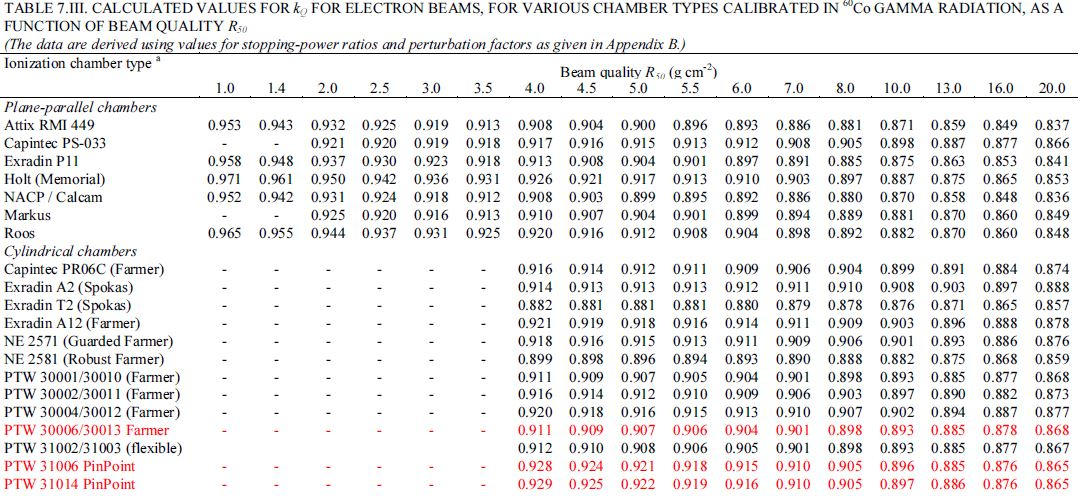
\includegraphics[width=0.9\textwidth]{Imagens/tabela73trs398.JPG}
			\caption{Valores calculados para o $K_Q$ para as câmaras de ionização calibradas em feixes de \ce{^{60}Co} }
			\label{fig:tabela73trs398}
		\end{figure}

		\begin{figure}[h]
			\centering
			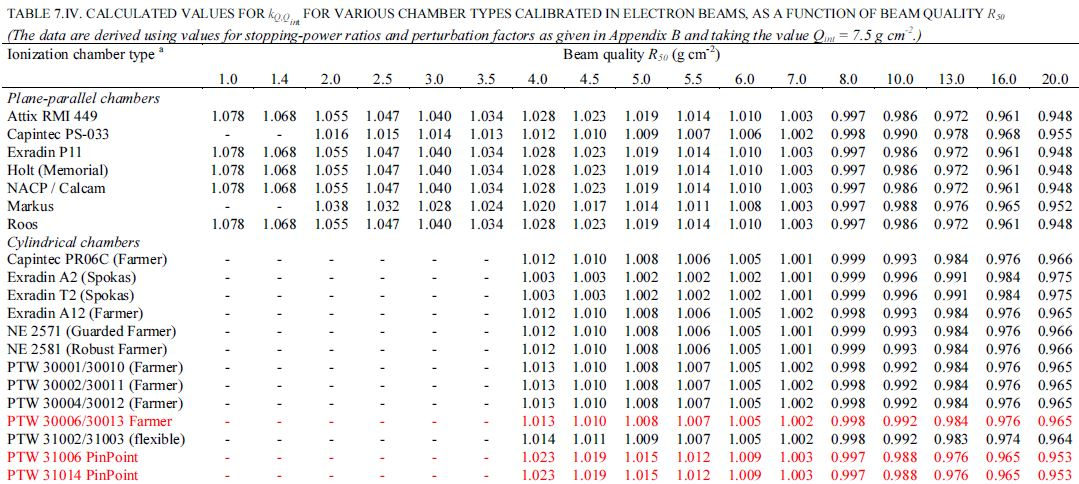
\includegraphics[width=0.9\textwidth]{Imagens/tabela74trs398.JPG}
			\caption{Valores calculados para o $K_{Q,Q_{int}}$ em função do $R_{50}$ = 7.5 \unit{g \cdot cm^{-2}} }
			\label{fig:tabela74trs398}
		\end{figure}
 
	\subsection*{Implementação}

	\subsubsection*{Fator de Calibração}

		Dependendo do Laboratório credenciado, o fator de calibração pode fornecido de quatro formas diferentes:

		\begin{enumerate}
			\item Pode ser fornecido o $N_{D,w,Q_0}$ para a qualidade de referência do \ce{^{60}Co} juntamente com o  $K_{Q,Q_0}$ caso o laboratório possua diferentes qualidades além da \ce{^{60}}, onde será possível fornecer o $K_{Q,Q_0}$ específico para a câmara calibrada e para os feixes do usuário;
			
			\item Pode ser fornecido o $N_{D,w,Q}$ específico para cada qualidade do usuário caso o laboratório possua as qualidades requeridas na calibração do usuário;
			
			\item Pode ser fornecido o $N_{D,w,Q_0}$ para a qualidade de referência do \ce{^{60}} e o fator de calibração $K_{Q,Q_0}$ pode ser determinado teoricamente para o tipo de câmara que será utilizada para outras qualidades de feixe; Este método ignora as variações de câmara para câmara em resposta com a energia de um determinado tipo de câmara, e os cálculos dependem das especificações da câmara fornecidas pelos fabricantes.
	
			\item Pode ser fornecido o $N_{D,w,Q_0}$ para a qualidade de referência do \ce{^{60}} e o fator de calibração $K_{Q,Q_0}$ pode ser obtido por um valor genérico fornecido por laboratórios padrão, obtidos através de dados experimentais feitos com o mesmo modelo da câmara que será utilizada na dosimetria. Esta opção não leva em consideração possíveis variações de câmara para câmara dentro de um determinado tipo de câmara, além de ter apenas os valores para as principais câmara comercializadas. 
		\end{enumerate}


	\subsubsection*{Características das Câmaras de Ionização}

	\begin{exemplo}[Câmaras Cilíndricas]
		\begin{itemize}[label=\textcolor{CarnationPink}{$\blacktriangleright$}]
			\item \textcolor{DarkTurquoise}{\LobsterTwo\textbf{Feixes:}}
				\begin{itemize}[label=\textcolor{CarnationPink}{$\star$}]
					\item Feixes de Radioterapia de média energia acima de 80 kV e HVL de 2 mm de Alumínio;
					\item \ce{^{60}Co};
					\item Fotons de Alta Energia;
					\item Feixes de elétrons com energias acima de aproximadamente 10 MeV;
					\item Feixes terapêuticos de prótons e ions pesados.
				\end{itemize}
			\item \textcolor{DarkTurquoise}{\LobsterTwo\textbf{Volume da cavidade:}} Entre 0.1 \unit{cm^3} e 1.0 \unit{cm^3};
			\item \textcolor{DarkTurquoise}{\LobsterTwo\textbf{Diâmetro interno:}} $\leq$ 7 mm;
			\item \textcolor{DarkTurquoise}{\LobsterTwo\textbf{Comprimento interno:}} $\leq$ 25 mm;
			\item \textcolor{DarkTurquoise}{\LobsterTwo\textbf{Uso:}} a câmara deve ser alinhada de tal forma que a fluência de radiação seja aproximadamente uniforme ao longo da seção transversal da cavidade da câmara e, portanto o comprimento da cavidade  define um limite do tamanho do campo mínimo no qual as medições podem ser feitas.
		\end{itemize}		 
	\end{exemplo}

	\begin{exemplo}[Câmaras de Placas Paralelas]
		\begin{itemize}[label=\textcolor{CarnationPink}{$\blacktriangleright$}]
			\item \textcolor{DarkTurquoise}{\LobsterTwo\textbf{Feixes:}}
				\begin{itemize}[label=\textcolor{CarnationPink}{$\star$}]
					\item Feixes de elétrons de todas as energias;
					\item Uso MANDATÓRIO para energias de elétrons abaixo de 10 MeV;
					\item Dosimetria de referência de feixes de fótons de alta energia somente quando é fornecida uma calibração em termos da dose absorvida na água para a qualidade do feixe do usuário;
					\item Feixes de prótons e íons pesados, principalmente para feixes com o SOBP estreito;
					\item Pode ser utilizada para fótons de baixa energia, com certas diferenças em sua construção
				\end{itemize}
			\item \textcolor{DarkTurquoise}{\LobsterTwo\textbf{Ponto efetivo:}} É definido na superfície interna da janela de entrada da câmara, no seu centro.
			\item \textcolor{DarkTurquoise}{\LobsterTwo\textbf{Raio da cavidade:}} $\leq$ 20 mm; (para reduzir a influência da não uniformidade radial do feixe)
			\item \textcolor{DarkTurquoise}{\LobsterTwo\textbf{Altura da cavidade:}}  $\leq$ 2 mm;
			\item \textcolor{DarkTurquoise}{\LobsterTwo\textbf{Eletrodo Coletor:}} Deve estar cercado por um eletrôdo de guarda com largura maior que 1.5 vezes a altura da cavidade;
			\item \textcolor{DarkTurquoise}{\LobsterTwo\textbf{Espessura da parede anterior:}} Deve ser de 0.1 \unit{g \cdot cm^{-2}} ou 1 mm de PMMA;
			\item \textcolor{DarkTurquoise}{\LobsterTwo\textbf{obs:}} é necessário que a cavidade de ar seja ventilada para que se equilibre rapidamente com a temperatura ambiente e a pressão do ar.
		\end{itemize}		
	\end{exemplo}

	\subsection*{Qualidades de Feixe para Aplicação do TRS-398 e TG-51}

	\begin{exemplo}
		\textcolor{DarkTurquoise}{\Large\LobsterTwo\textbf{TRS-398}}
		\begin{itemize}
			\item Raios-x de baixa energia com potenciais geradores de até 100 kV e HVL de 3 mm Al (o limite inferior é determinado pela disponibilidade de padrões para dada energia);
			\item Raios X de média energia com potenciais geradores acima de 80 kV e HVL de 2 mm Al;
			\item Radiação gama \ce{^{60}Co};
			\item Fótons de alta energia gerados por elétrons acelerados com energias no intervalo de 1 MeV a 50 MeV, com valores de $TPR_{20,10}$ entre 0.50 e 0.84;
			\item Elétrons no intervalo de energia 3 MeV a 50 MeV, com profundidade de ``meio valor'', $R_{50}$, entre 1 g $cm^{-2}$ e 20 g $cm^{-2}$;
			\item Prótons no intervalo de energia de 50 MeV a 250 MeV, com alcance prático, $R_p$, entre 0.25 g $cm^{-2}$ e 25 g $cm^{-2}$;
			\item Íons pesados com Z entre 2 (He) e 18 (Ar) tendo um alcance prático em água, $R_p$, de 2 g $cm^{-2}$ a 30 g $cm^{-2}$ (para íons de carbono isso corresponde a uma faixa de energia de 100 MeV/u a 450 MeV/u, onde u é a unidade de massa atômica).
		\end{itemize}

		\textcolor{DarkTurquoise}{\Large\LobsterTwo\textbf{TG-51}}
		\begin{itemize}
			\item Qualidades de fótons com energia nominal variando entre o \ce{^{60}Co} (média de 1.25 MeV) e 50 MV;
			\item Qualidades de elétrons com energia nominal variando entre 4 MeV e 50 MeV. 
		\end{itemize}
		
	\end{exemplo}

    \section{Dosimetria de Feixes de Fótons de Megavoltagem}

    Os principais protocolos utilizados para a determinação da dose absorvida na água são: AAPM TG-51 (Protocol for Clinical Reference Dosimetry of High-Energy Photon and Electron Beams) e  o IAEA TRS-398 (Absorbed Dose Determination in External Beam Radiotherapy).  

    Ambos protocolos utilizam uma câmara cilíndrica para determinar a dose absorvida na água para feixes de fótons MV.  A leitura da carga deve ser corrigida pela temperatura, pressão, recombinação iônica e polaridade. Essas correções são feitas para considerar a pertubação no meio devido a presença da câmara. \textcolor{MediumOrchid}{\textit{\textbf{Ambos os protocolos utilizam um campo de referência 10 cm x 10 cm para realização das medidas.}}}.

    No geral, os protocolos realizam as medidas em uma certa \textcolor{MediumOrchid}{\textit{\textbf{profundidade de referência}}} e corrige a leitura pela PDP para obter a \textcolor{MediumOrchid}{\textit{\textbf{dose na profundidade de dose máxima}}}. Isso é feito para que a leitura possa ser realizada em uma profundidade onde a PDP pode ser determinada com maior exatidão, pois qualquer desvio da posição da câmara em relação à profundidade exata onde ocorre a dose máxima pode levar a erros de calibração significantes. A \ref{fig:condicoesReferenciasTPR2010jpg} apresenta as condições de referência para determinação da qualidade do feixe através do protocolo TRS-398, e a \ref{fig:condicoesReferenciasDoseFotons} apresenta as condições de referência para determinação da dose absorvida na água para feixes de fótons do mesmo protocolo.

    A equação geral para obter a dose absorvida na água a partir da leitura de carga de uma câmara de ionização medida com um eletrômetro é dada por:

  		$$D_{w}(z) = M \; N_{D,w} \; K_{pol} \; K_{ion} \; K_{T,P} \; K_{Q,Q_0}$$

	\begin{exemplo}[onde:]
		\begin{itemize}[label=\textcolor{CarnationPink}{$\star$}]
			\item \textbf{\textcolor{DarkTurquoise}{$D_{w}(z)$}}: É a dose absorvida na água na profundidade Z;
			\item \textbf{\textcolor{DarkTurquoise}{$M$}}: é a leitura da câmara de ionização corrigida pela calibração do eletrômetro
			\item \textbf{\textcolor{DarkTurquoise}{$N_{D,w}$}}: É o fator de calibração para a dose absorvida na água para a energia do \ce{^{60}Co};
			\item \textbf{\textcolor{DarkTurquoise}{$K_{pol}$}}: É o fator de correção de polaridade; Este valor é geralmente menor que 1\% da unidade. Ele deve se manter estável de ano em ano e qualquer desvio maior que 0.5\% do valor médio da corrente deve ser investigado. Para novas câmaras, ele deve ser medido várias vezes para estabelecer consistência; 
			\item \textbf{\textcolor{DarkTurquoise}{$K_{ion}$}}: É o fator de recombinação iônica. Este valor é normalmente menor que 1.01 e o TG-51 recomenda não utilizar a câmara cas este fator seja maior que 5\%. 
			\item \textbf{\textcolor{DarkTurquoise}{$K_{T,P}$}}: É o fator de correção para a densidade do ar, que corrige a leitura com respeito a temperatura e pressão. 
			\item \textbf{\textcolor{DarkTurquoise}{$K_{Q,Q_0}$}}: É o fator de correção da qualidade do feixe, que corrige a leitura para o feixe avaliado versos o feixe do \ce{^{60}Co} para o qual o fator de calibração foi determinado. o $K_{Q,Q_0}$ é específico para a energia do feixe que está sendo medida e da câmara de ionização que está sendo utilizada para realizar as medidas. Seus valores variam de 1 até aproximadamente 0.96 para feixes MV.
		\end{itemize}
	\end{exemplo}

	\begin{exemplo}[Fator de Correção De Polaridade]

		\begin{itemize}
			\item \textcolor{DarkTurquoise}{\Large\LobsterTwo\textbf{TRS-398}}
			
				$$K_{pol} = \frac{\left\lvert M_+ \right\rvert + \left\lvert M_- \right\rvert }{2M}$$

				onde,
				\begin{itemize}[label=\textcolor{CarnationPink}{$\star$}]
					\item $M_+$ é a leitura do eletrômetro com a polaridade positiva;
					\item $M_-$ é a leitura do eletrômetro com a polaridade negativa;
					\item $M$ é a leitura do eletrômetro na polaridade usada na rotina (positiva ou negativa);
				\end{itemize}

			\item \textcolor{DarkTurquoise}{\Large\LobsterTwo\textbf{TG-51}}
			
				$$K_{pol} = \left|\frac{ M_{raw}^+ - M_{raw}^- }{2M_{raw}}\right|$$

				onde,
				\begin{itemize}[label=\textcolor{CarnationPink}{$\star$}]
					\item $M_{raw}^+$ é a leitura quando cargas positivas são coletadas;
					\item $M_{raw}^-$ é a leitura quando cargas negativas são coletadas;
					\item $M_{raw}$ é a leitura das cargas comumente utilizadas na rotina.
				\end{itemize}

			\item \textcolor{MediumOrchid}{\textbf{\textit{Obs}:}} O valor do $K_{pol}$ poderá variar acima ou abaixo de 1, dependendo da polaridade definida como padrão para as medidas mas não deve exceder uma diferença de $\pm$ 1\%. Se a câmara for utilizada para calibração da mesma qualidade de feixe, não será necessário um fator de correção de polarização. Este efeito é pequeno e varia com a energia de modo que se o $K_{pol}$ for conhecido para a qualidade de referência utilizada na calibração $(K_{pol})_{Q_0}$ então $K_{pol}$ deverá ser dado pela razão $(K_{pol})_{Q}/(K_{pol})_{Q_0}$ caso os valores de $K_{pol}$ excedam 0.3\% para feixes acima de 6MV ou feixes de \ce{^{60}Co}.
		\end{itemize}
		
	\end{exemplo}
	
	\begin{exemplo}[Fator de Recombinação Iônica]
		\begin{itemize}
			\item \textcolor{DarkTurquoise}{\Large\LobsterTwo\textbf{TRS-398:}}
			
			Para feixes pulsados:

				$$K_{ion} - 1 = \frac{M_1/M_2 - 1}{V_1/V_2 - 1}$$
			ou
				$$K_{ion} = a_0 + a_1\frac{M_1}{M_2} + a_2\left(\frac{M_1}{M_2}\right)^2$$

			Para o Cobalto-60, onde existe radiação contínua

				$$K_{ion} - 1 = \frac{(V_1/V_2)^2- 1}{(V_1/V_2)^2 - (M_1/M_2)^2}$$

			onde,
			\begin{itemize}[label=\textcolor{CarnationPink}{$\star$}]
				\item $V_1$ e $V_2$ São diferentes tensões de polarização;
				\item $M_1$ é a leitura da carga medida com a tensão de polarização $V_1$;
				\item $M_2$ é a leitura da carga medida com a tensão de polarização $V_2$;
				\item $a_0$, $a_1$ e $a_2$ são coeficientes (constantes) fornecidas no documento para feixes pulsados.
				\item \textcolor{MediumOrchid}{\textbf{Obs:} Este método assume uma dependencia linear entre 1/M e 1/V o que pode não ocorrer com câmaras de placas paralelas no intervalo de voltagem utilizado no método de duas voltagens.}
			\end{itemize}

			\item \textcolor{DarkTurquoise}{\Large\LobsterTwo\textbf{TG-51:}}
			
			Para radiação pulsada:
				$$K_{ion} = \frac{1 - V_H/V_L}{M_{raw}^H/M_{raw}^L - V_H/V_L}$$

			Para radiação contínua:

				$$K_{ion} = \frac{1 - (V_H/V_L)^2}{M_{raw}^H/M_{raw}^L - (V_H/V_L)^2}$$

			onde,
			\begin{itemize}[label=\textcolor{CarnationPink}{$\star$}]
				\item $V_H$ é a voltagem de polarização normal (sempre a maior);
				\item $V_L$ é a voltagem 2 vezes menor que a voltagem normal;
				\item $M_{raw}^H$ é a leitura para a voltagem $V_H$;
				\item $M_{raw}^L$ é a leitura para a voltagem $V_L$;
			\end{itemize}

			\item \textcolor{MediumOrchid}{\textbf{Obs:}} A recombinação iônica depende principalmente da dose por pulso e; portanto esse fator será diferente para feixes FFF. É necessário que o fator de correção seja menor que 1.05, caso contrário outra câmara deverá ser utilizada.
		\end{itemize}
	\end{exemplo}

	\begin{exemplo}[Fator de Correção de Temperatura e Pressão]
		\begin{itemize}
			\item \textcolor{DarkTurquoise}{\Large\LobsterTwo\textbf{TRS-398:}}

				$$K_{T,P} = \frac{273.2 + T}{273.2 + T_0} \times \frac{P_0}{P}$$
				$$K_{T,P} = \frac{273.2 + T}{273.2 + \ang{20}C} \times \frac{101.3\;kPa}{P}$$

			onde,
			\begin{itemize}[label=\textcolor{CarnationPink}{$\star$}]
				\item $T_0$ é a temperatura de referência estabelecida como \ang{20}C;
				\item $T$ é a temperatura da água no momento da medida dada em \unit{\celsius}.
				\item $P_0$ é a pressão de referência definida como 101.3 kPa;
				\item $P$ é a pressão atmosférica no momento da medida, dada em kPa;
			\end{itemize}

			\item \textcolor{DarkTurquoise}{\Large\LobsterTwo\textbf{TG-51:}}
			
				$$K_{T,P} = \frac{273.2 + T}{273.2 + T_0} \times \frac{P_0}{P}$$
				$$K_{T,P} = \frac{273.2 + T}{273.2 + \ang{22.0}C} \times \frac{101.3\;kPa}{P}$$

			onde,
			\begin{itemize}[label=\textcolor{CarnationPink}{$\star$}]
				\item $T_0$ é a temperatura de referência estabelecida como \ang{22}C;
				\item $T$ é a temperatura da água no momento da medida dada em \unit{\celsius}.
				\item $P_0$ é a pressão de referência definida como 101.3 kPa;
				\item $P$ é a pressão atmosférica no momento da medida, dada em kPa;
			\end{itemize}
			\item \textcolor{MediumOrchid}{\textbf{Obs:}} Não são necessárias correções de umidade se o fator de calibração foi referido a uma umidade relativa do ar de 50\% e é usado em uma umidade relativa  do ar variando entre 20\% e 80\%.
		\end{itemize}
	\end{exemplo}

	\begin{exemplo}[Fator de Qualidade do Feixe]
		\begin{itemize}
			\item \textcolor{DarkTurquoise}{\Large\LobsterTwo\textbf{TRS-398:}} 
			
			É fornecida uma tabela de valores para várias câmaras de ionização em uma faixa de energias de feixe. A qualidade do feixe é especificada pela relação entre a TPR a 20 cm de profundidade e a TPR a 10 cm de profundidade para o tamanho do campo de referência, ou seja, $TPR_{20,10}$. Os valores da TPR podem ser medidos diretamente ou calculados a partir de medidas da PDP utilizando a equação empírica: $$TPR_{20,10} = 1.2661* (PDP(20)/PDP(10)) - 0.0595$$ Recomenda-se o uso de um valor medido em vez de um valor genérico obtido pela equação acima.
			

			\item \textcolor{DarkTurquoise}{\Large\LobsterTwo\textbf{TG-51:}} 
			
			É fornecido uma tabela de valores para várias câmaras de ionização em uma faixa de energias de feixe. A qualidade do feixe é especificada pela PDP a 10 cm de profundidade, SSD de 100 cm com contaminação eletrônica removida ou PDD(10)x para energias $\geq$ 10 MV. Para medir a PDP da componente de fóton, uma folha de chumbo fina (1 mm) é colocada a 50 cm da fonte para eliminar a contaminação do feixe com elétrons em energias de 10 MV ou mais. Esta folha de chumbo é usada apenas para medida da PDP e deve ser removida para a medida do output.
		\end{itemize}
	\end{exemplo}

	\begin{exemplo}[Ponto de Referência da Câmara de Ionização]
		\begin{itemize}
			\item \textcolor{DarkTurquoise}{\Large\LobsterTwo\textbf{TRS-398:}}
			
			O ponto de referência da câmara, definido no centro da câmara cilíndrica é colocado na profundidade de referência;
			
			\item \textcolor{DarkTurquoise}{\Large\LobsterTwo\textbf{TG-51:}}
			
			O ponto de referência da câmara, definido no centro da câmara cilíndrica é colocado na profundidade de referência;
		\end{itemize}
	\end{exemplo}

	\begin{exemplo}[Fator de Correção do Eletrômetro]
		Será necessário um fator de correção para o eletrômetro ($K_{elec}$) sempre que a câmara for calibrada separadamente do eletrômetro; Deste modo, o laboratório deverá fornecer separadamente um fator de correção para o eletrômetro além do $N_{D,w}$. 
	\end{exemplo}


	Alguns Laboratórios de calibração estão se direcionando para oferecer calibrações para outras qualidades de feixe além da do \ce{^{60}Co}. Isto tem uma vantagem de que o $K_{Q,Q_0}$ determinado será para a câmara específica que está sendo utilizada na medida e não para um valor de $K_{Q,Q_0}$ genérico dado para o modelo da câmara. Para isto, pode-se adotar duas estratégias diferentes:

	\begin{enumerate}
		\item O laboratório de calibração determinar o $N_{D,w}$ para a câmara juntamente com uma série de valores de $K_{Q,Q_0}$ em toda a gama de qualidades de feixe, incluindo os feixes de elétrons. Isto tem a vantagem de que, como não se espera que a dependência energética da câmara mude, as calibrações da câmara exigirão apenas a determinação do $N_{D,w}$ na qualidade de referência $Q_0$.
		\item O laboratório determinar vários valores de $N_{D,w}$, eliminando a necessidade de utilizar o $K_{Q,Q_0}$;
	\end{enumerate}

	\begin{figure}[h]
		\centering
		\fcolorbox{DarkTurquoise}{white}{%
			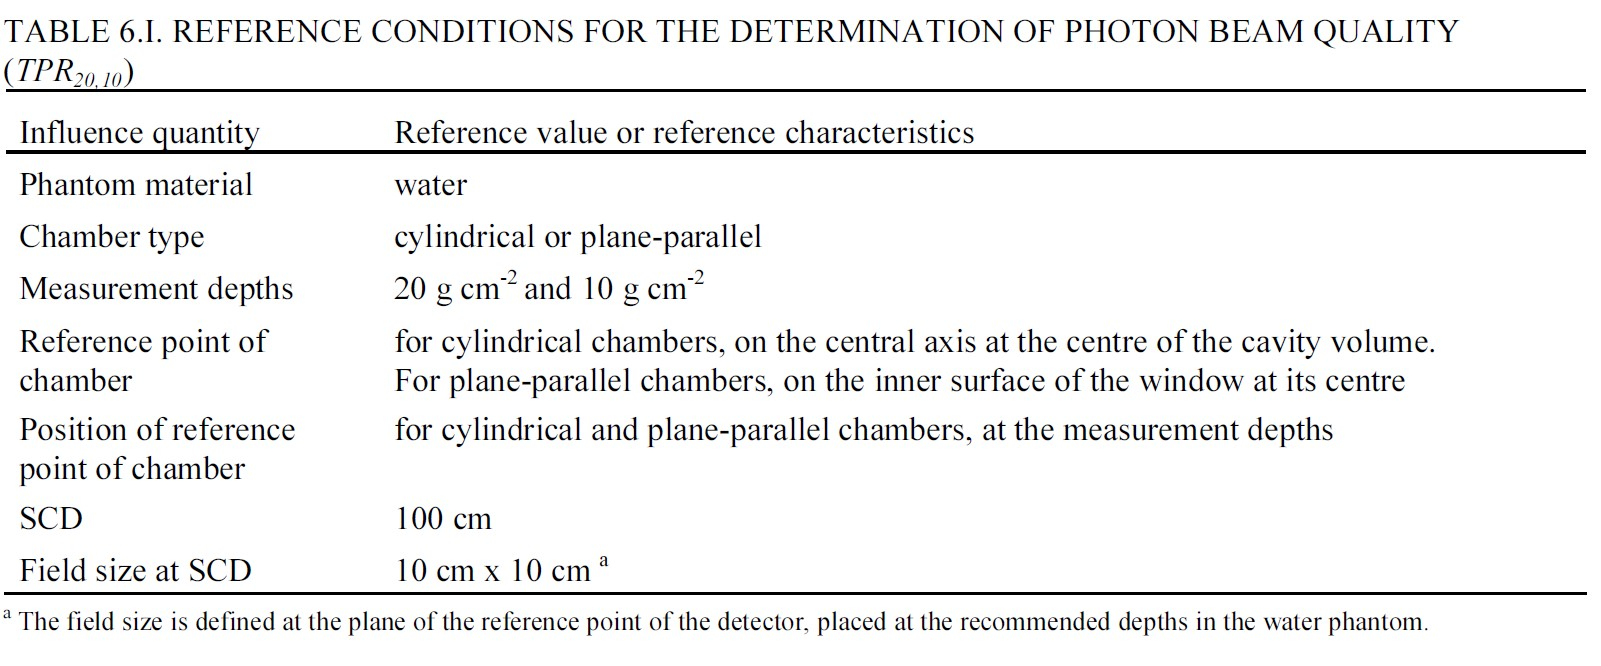
\includegraphics[width=0.8\textwidth]{Imagens/condicoesReferenciasTPR2010jpg.jpg}
		}%
		\caption{Condições de Referência para a Determinação da Qualidade do Feixe de fótons através do TPR20,10}
		\label{fig:condicoesReferenciasTPR2010jpg}
	\end{figure}

	\begin{figure}[h]
		\centering
		\fcolorbox{DarkTurquoise}{white}{%
			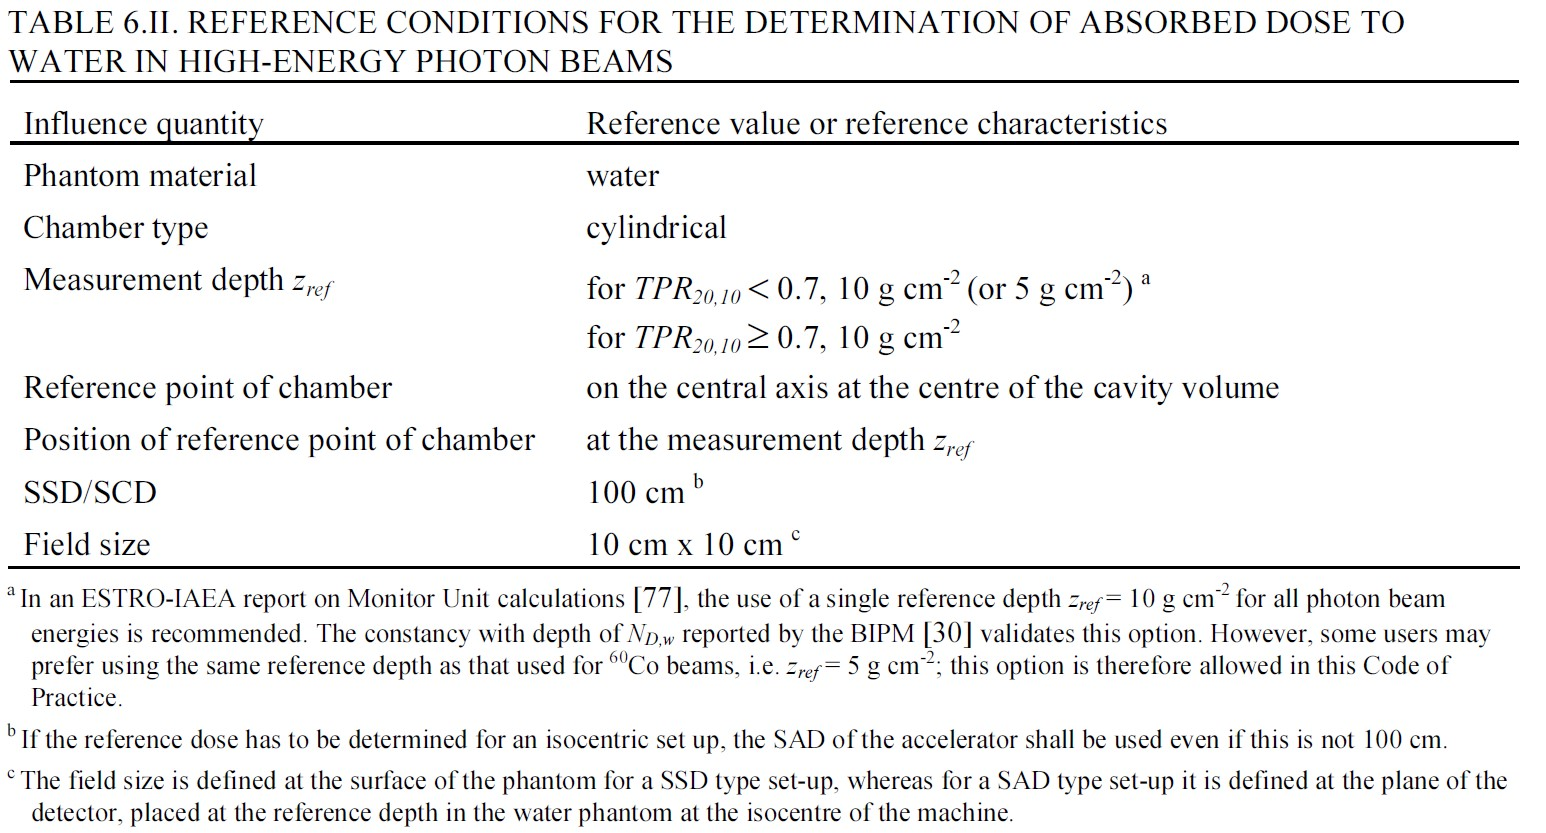
\includegraphics[width=0.8\textwidth]{Imagens/condicoesReferenciasDoseFotons.jpg}
		}%
		\caption{Condições de referência para a determinação da dose absorvida na água para feixes de fótons}
		\label{fig:condicoesReferenciasDoseFotons}
	\end{figure}

	\subsection{Feixes de MV Não-Padrão}

		São os feixes vindos da Tomoterapia, GammaKnife, CyberKnife onde \textcolor{MediumOrchid}{\textbf{\textit{não é possível definir um campo de referência 10 cm x 10 cm}}} ou \textcolor{MediumOrchid}{\textbf{\textit{não é possível estabelecer a SSD de referência}}} utilizadas nos protocolos. O TG-21 é utilizado nos casos em que não é possível utilizar um phantom de água, como o GammaKnife, onde a determinação da dose é feita no ar. Outro protocolo utilizado no GammaKnife é o TG-178 ``\textit{Gamma Stereotactic Radiosurgery Dosimetry and Quality Assurance}'' onde é aplicado o protocolo ALF para dosimetria nesses equipamentos. Além disto o detector aplicado deve ser definido adequadamente de modo que que seja pequeno o suficiente para que a diferença percentual no gradiente de dose que atravessa o volume do detector seja muito pequena. \textcolor{MediumOrchid}{\textbf{\textit{Fatores de correção}}} devem ser aplicados em feixes cujo \textcolor{MediumOrchid}{\textbf{\textit{gradiente de dose é inerente do feixe}}}, como em feixes FFF. Maquinas que utilizam MRI devem estabelecer um fator de correção para leitura da câmara que dependerá da intensidade do campo magnético aplicado.
	

	\section{Feixes de Elétrons}

	Para a dosimetria de feixes de elétrons, são feitas as seguintes recomendações:

		\begin{itemize}
			\item \textcolor{DarkTurquoise}{\Large\LobsterTwo\textbf{TRS-398}}: É necessário o uso de câmaras de ionização de placas paralelas para todas as energias de elétrons embora uma câmara cilíndrica possa ser utilizadas em feixes com $R_{50} \geq 4\;cm$ na água ($E_0 \sim 10\; MeV$). 
			\item \textcolor{DarkTurquoise}{\Large\LobsterTwo\textbf{TG-51}}: é necessário a utilização de câmaras de placas paralelas para feixes de elétrons com energia $\leq$ 6 MeV e é recomendado seu uso para energias menores que 10 MeV.
		\end{itemize}

	A qualidade do feixe de elétrons é definida como sendo a \textcolor{MediumOrchid}{\textbf{\textit{profundidade da curva de isodose de 50\%}}}. Caso uma câmara cilíndrica seja utilizada para determinar a PDP do feixe de elétrons, a curva deve ser deslocada para cima $0.5\cdot r_{cav}$ (descer o centro da câmara 0.5 x raio para baixo do ponto de análise) para considerar o ponto efetivo de medida e a curva de ionização resultante deve ser convertida na curva de PDP através da razão dos poderes de freamento. Para converter a \textcolor{MediumOrchid}{\textbf{\textit{curva de ionização em PDP}}} na profundidade da isodose de 50\% utiliza-se as seguintes relações:

		\begin{equation}
			R_{50} = 
			\begin{cases}
				(1.028 \times I_{50}) - 0.06 \;cm  & \text{ para }  I_{50} \leq 10 \; cm \text{ na agua}, \\
				\\
				(1.059 \times I_{50}) - 0.37\;cm  & \text{ para } I_{50} > 10\;cm \text{ na agua}
			\end{cases}
		\end{equation}


	Também é possível derivar o $R_{50}$ mais diretamente utilizando medidas através de um diodo, que não requer um \textit{``shift''} na isodose e nem correções para o poder de freamento. 

	A profundidade de referência para todos os protocolos referidos, determinam que a profundidade de referência é dada por:

		\begin{equation}
			d_{\text{ref}} = (0.6 \times R_{50}) - 0.1 (cm)
		\end{equation}
		

	A dose na profundidade de dose máxima ($d_{\text{max}}$) é então determinada utilizando a PDP medida para o feixe.

	De acordo com o TRS-398 é preferível utilizar um phantom de água, porém para feixes com $R_{50} < 4 \; cm$ pode-se utilizar um phantom de plástico. Nestes casos é necessário utilizar um fator de escala para corrigir o posicionamento da câmara.  A \ref{fig:condicoesReferenciasR50}, \ref{fig:condicoesReferenciasDoseEletrons} e \ref{fig:fatorEscalaPhantons} mostram as condições de referência para a determinação do $R_{50}$, dose absorvida na água e fator de escala, respectivamente, para feixes de elétrons calibrados de acordo com o protocolo TRS-398.
	
	\subsection*{Calibração Cruzada}
	
	Se for utilizada uma câmara de placas paralelas sem um fator de calibração fornecido por um laboratório padrão primário, deverá ser realizada a \textcolor{MediumOrchid}{\textbf{\textit{calibração cruzada}}} desta câmara com uma \textcolor{MediumOrchid}{\textbf{\textit{câmara cilíndrica calibrada}}} em um laboratório padrão.

	Para este fim, é necessário utilizar a maior energia de elétrons disponível, preferencialmente que o  $R_{50} \geq 7\; g\cdot cm^{-2}$ (Equivalente a $E_0 > 16 \; MeV$). O fator de calibração em termos da dose absorvida de água para a câmara sob calibração, na qualidade de calibração cruzada $Q_{cross}$, é dado por:

	$$N_{D,w,Q_{cross}}^{x} = \frac{M_{Q_{cross}}^{ref}}{M_{Q_{cross}}^{x}} \cdot N_{D,w,Q_0}^{ref}\cdot k_{Q_{cross},Q_0}^{ref}$$

	\begin{exemplo}[onde:]
		\begin{itemize}
			\item \textcolor{DarkTurquoise}{$N_{D,w,Q_{cross}}^{x}$}: é o fator de calibração cruzada para a câmara de placas paralelas sendo calibrada;
			\item \textcolor{DarkTurquoise}{$M_{Q_{cross}}^{ref}$}: é a leitura obtida com a câmara de referência posicionada em $z_{ref}$ e corrigida pelos fatores de influência;
			\item \textcolor{DarkTurquoise}{$M_{Q_{cross}}^{x}$}: é a leitura com a câmara de placas paralelas sendo calibrada posicionada em $z_{ref}$ e corrigida pelos fatores de influência;
			\item \textcolor{DarkTurquoise}{$N_{D,w,Q_0}^{ref}$}: é o fator de calibração dado em termos da dose absorvida na água para a câmara de referência; e
			\item \textcolor{DarkTurquoise}{$ k_{Q_{cross},Q_0}^{ref}$}: é o fator de correção para a qualidade do feixe para o qual a câmara de referência está sendo utilizada, dado por $$k_{Q_{cross},Q_0}^{ref} = \frac{k_{Q_{cross},Q_{int}}^{ref}}{k_{Q_0, Q_{int}}^{ref}}$$
		\end{itemize}
	\end{exemplo}

	A câmara pode então ser utilizada para determinação da dose absorvida na água para uma qualidade Q através da equação:

	$$D_{w,Q} = M_{Q}^{x}\cdot N_{D,w,Q_{cross}}^{x} \cdot k_{Q,Q_{cross}}^{x} $$

	onde $$k_{Q,Q_{cross}}^{x} = \frac{k_{Q,Q_{int}}^{x}}{k_{Q_{cross}, Q_{int}}^{x}}$$

	\begin{figure}[h]
		\centering
		\fcolorbox{DarkTurquoise}{white}{%
			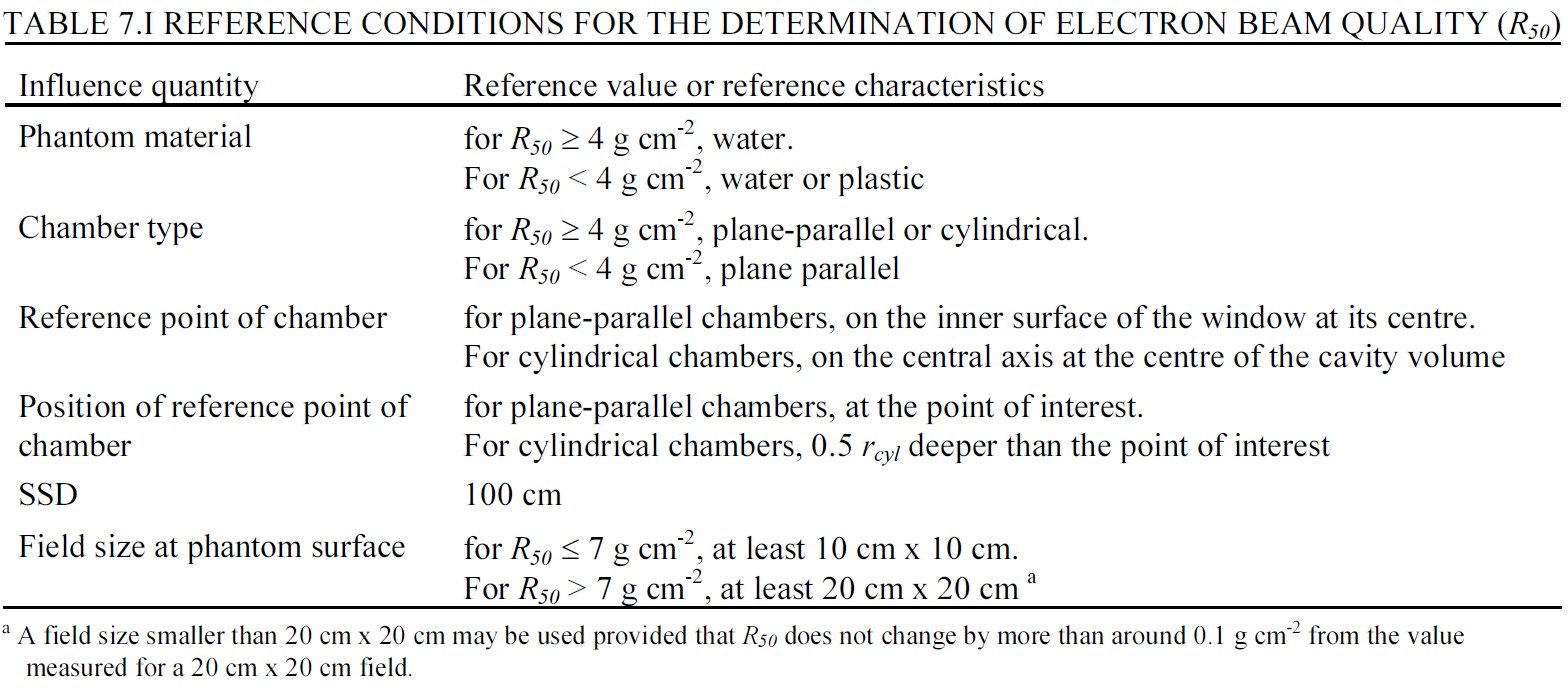
\includegraphics[width=0.8\textwidth]{Imagens/condicoesReferenciasR50.jpg}
		}%
		\caption{Condições de referência para determinação do R50 de acordo com o TRS-398}
		\label{fig:condicoesReferenciasR50}
	\end{figure}

	\begin{figure}[h]
		\centering
		\fcolorbox{DarkTurquoise}{white}{%
			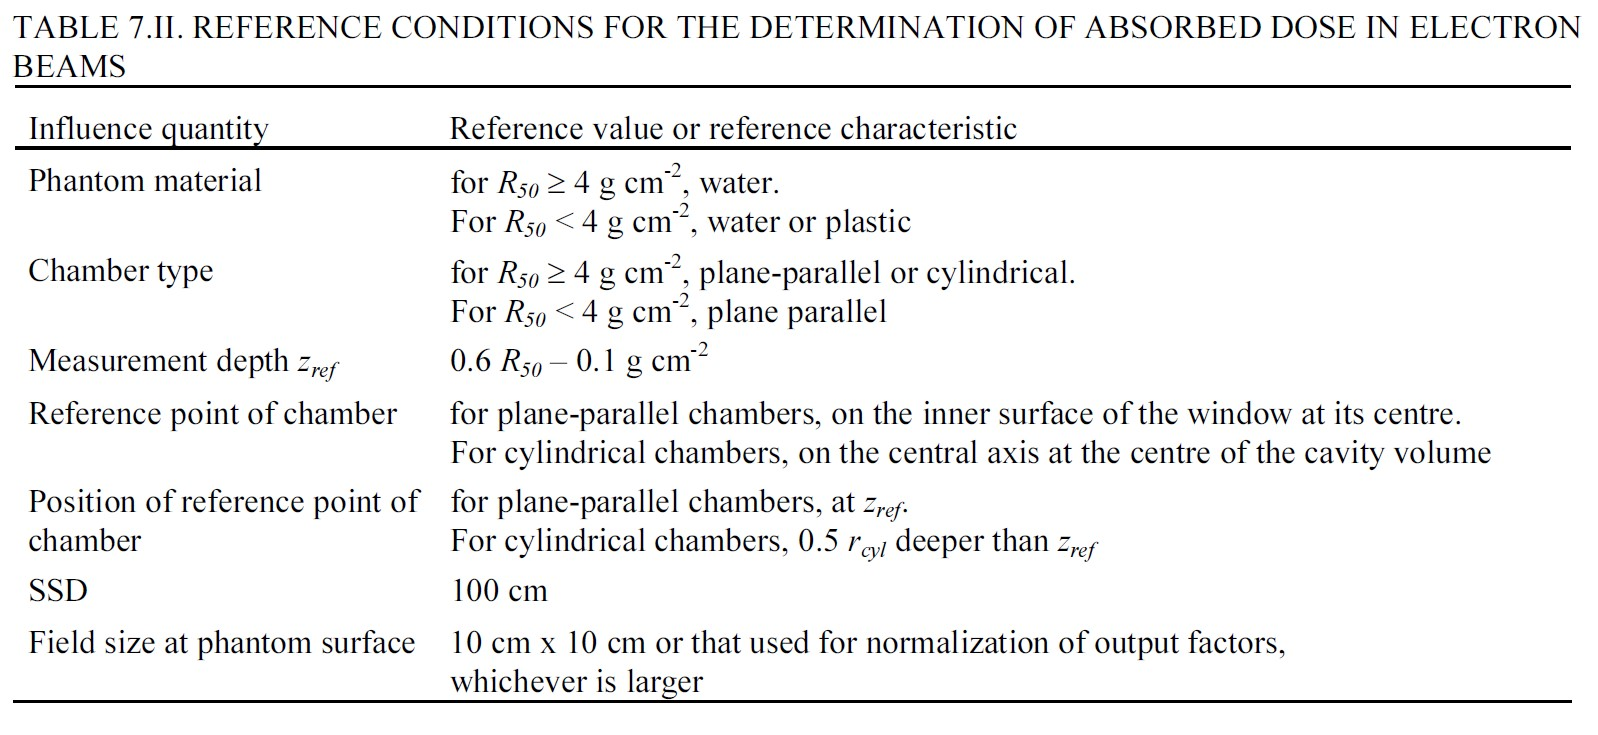
\includegraphics[width=0.8\textwidth]{Imagens/condicoesReferenciasDoseEletrons.jpg}
		}%
		\caption{Condições de referência para a determinação da dose absorvida na água para feixes de elétrons.}
		\label{fig:condicoesReferenciasDoseEletrons}
	\end{figure}

	\begin{figure}[h]
		\centering
		\fcolorbox{DarkTurquoise}{white}{%
			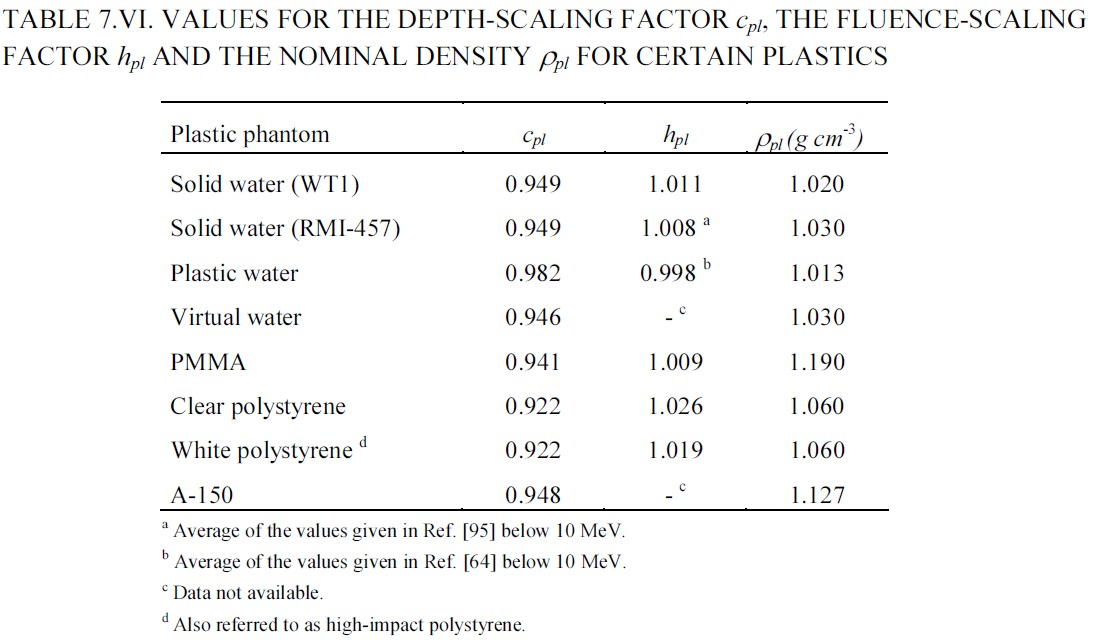
\includegraphics[width=0.8\textwidth]{Imagens/fatorEscalaPhantons.jpg}
		}%
		\caption{Fator de escala para determinação da profundidade de referência para diferentes materiais}
		\label{fig:fatorEscalaPhantons}
	\end{figure}

\section{Dosimetria em Feixes KV}

	O \textcolor{MediumOrchid}{\textbf{\textit{TG-61}}}, ``\textbf{\textit{AAPM Protocol for 40-300 kV X-ray Beam Dosimetry in Radiotherapy and Radiobiology}}'' e o IAEA TRS-398 descrevem a metodologia usada para medir a dose absorvida para feixes de fótons kV. 
	
	O  TG-61 é baseado se baseia na \textcolor{MediumOrchid}{\textbf{\textit{calibração do kerma no ar de uma câmara de ionização}}}. Este protocolo pode ser aplicado em uma faixa kV variando de \textcolor{MediumOrchid}{\textbf{\textit{40 kV a 300 kV}}}. Podem ser utilizadas \textcolor{MediumOrchid}{\textbf{\textit{câmaras de placas paralelas}}} ou \textcolor{MediumOrchid}{\textbf{\textit{câmaras cilíndricas}}} para feixes \textcolor{MediumOrchid}{\textbf{\textit{$>$ 70 kV}}}, com o \textcolor{MediumOrchid}{\textbf{\textit{ponto efetivo}}} de medida definido como o \textcolor{MediumOrchid}{\textbf{\textit{centro da cavidade de ar}}}. Uma \textcolor{MediumOrchid}{\textbf{\textit{câmara de placas paralelas}}} com uma \textcolor{MediumOrchid}{\textbf{\textit{janela de entrada fina}}} deve ser usada para feixes com energia  \textcolor{MediumOrchid}{\textbf{\textit{$<$ 70 kV}}}. \textcolor{MediumOrchid}{\textbf{\textit{Placas plásticas finas}}} podem ser necessárias para \textcolor{MediumOrchid}{\textbf{\textit{remover a contaminação de elétrons}}} e fornecer o buildup adequado. Para feixes com energia \textcolor{MediumOrchid}{\textbf{\textit{$<$ 100 kV}}}, a medida deve ser feita no \textcolor{MediumOrchid}{\textbf{\textit{ar}}} e deve ser utilizado um  \textcolor{MediumOrchid}{\textbf{\textit{fator de retroespalhamento}}}  para contabilizar o espalhamento no phantom. No TG-61 é fornecida uma tabela de valores de retroespalhamento com base na SSD e na qualidade do feixe. A qualidade do feixe é baseada na \textcolor{MediumOrchid}{\textbf{\textit{camada semi-redutora (HVL)}}} em \textcolor{MediumOrchid}{\textbf{\textit{Al}}} ou \textcolor{MediumOrchid}{\textbf{\textit{Cu}}}. Feixes com energias \textcolor{MediumOrchid}{\textbf{\textit{superiores a 100 kV}}} devem ser medidos na \textcolor{MediumOrchid}{\textbf{\textit{água}}} a uma profundidade de referência de \textcolor{MediumOrchid}{\textbf{\textit{2 cm}}}. Devem ser feitas correções para recombinação iônica, polaridade, calibração do eletrômetro e densidade do ar. Além disso, são feitas correções para o efeito final do temporizador e o efeito da haste da câmara.

	As seções 8 e 9 DO TRS-398 descrevem a metodologia para calibração de feixes de kV de baixa energia e de média energia. A \textcolor{MediumOrchid}{\textbf{\textit{seção 8}}} diz respeito à dosimetria de referência e relativa em feixes de raios X de baixa energia classificados como os feixes com \textcolor{MediumOrchid}{\textbf{\textit{HVL de até 3 mm de alumínio e potenciais geradores de até 100 kV}}}. A seção 9 diz respeito à dosimetria relativa e de referência de feixes de raios X de média energia classificadas como os feixes com \textcolor{MediumOrchid}{\textbf{\textit{HVL superiores a 2 mm de alumínio e potenciais geradores superiores a 80 kV}}}.
	
	Para feixes \textcolor{MediumOrchid}{\textbf{\textit{kV de baixa energia}}}, recomenda-se uma \textcolor{MediumOrchid}{\textbf{\textit{câmara de placas paralelas}}}. Se a câmara for usada com \textcolor{MediumOrchid}{\textbf{\textit{raios X de 50 kV ou acima}}}, geralmente será \textcolor{MediumOrchid}{\textbf{\textit{necessário adicionar lâminas}}} de material semelhante à janela da câmara para \textcolor{MediumOrchid}{\textbf{\textit{garantir o buildup}}} total. As espessuras necessárias podem ser vistas na \ref{fig:kvEspessuraBuildup}.

	\begin{figure}[h]
		\centering
		\fcolorbox{DarkTurquoise}{white}{%
			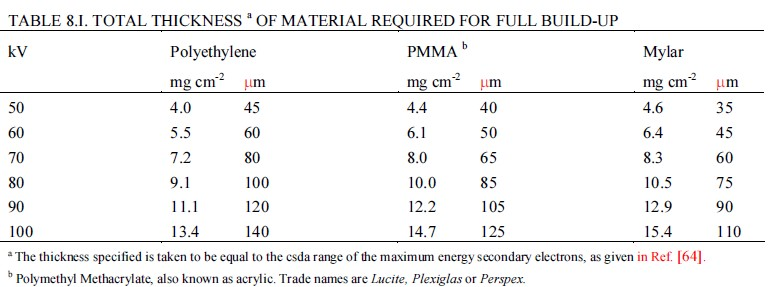
\includegraphics[width=0.8\textwidth]{Imagens/kvEspessuraBuildup.jpg}
		}%
		\caption{Espessura total de material para fornecer o completo buildup}
		\label{fig:kvEspessuraBuildup}
	\end{figure}
	
	O \textcolor{MediumOrchid}{\textbf{\textit{ponto de referência}}} é a \textcolor{MediumOrchid}{\textbf{\textit{superfície externa}}} da \textcolor{MediumOrchid}{\textbf{\textit{câmara de placas paralelas}}} ou a superfície externa das \textcolor{MediumOrchid}{\textbf{\textit{placas de plástico}}}, se forem usadas para garantir o buildup adequado. Como o ponto de referência está na superfície externa da câmara (ou placas) e deve estar nivelado com a superfície do phantom, os \textcolor{MediumOrchid}{\textbf{\textit{phantoms de plástico são recomendados}}} devido à dificuldade de se fazer isso em um phantom de água. A \textcolor{MediumOrchid}{\textbf{\textit{HVL em alumínio}}} é usada como o índice de qualidade do feixe, embora haja discussão de que isso não é totalmente preciso e introduz até cerca de 1.5\% de incerteza.
	
	Para feixes \textcolor{MediumOrchid}{\textbf{\textit{kV de média energia}}} deve ser utilizada uma \textcolor{MediumOrchid}{\textbf{\textit{câmara cilíndrica com volume entre 0.1 cc e 1.0 cc}}}. O \textcolor{MediumOrchid}{\textbf{\textit{ponto de referência}}} é localizado no \textcolor{MediumOrchid}{\textbf{\textit{centro do volume}}} e deve ser colocado a \textcolor{MediumOrchid}{\textbf{\textit{2 cm}}} de profundidade na água. Os fatores de correção da qualidade do feixe para feixes kV no TRS-398 usam uma metodologia de dose absorvida para água. Como a dose absorvida nas calibrações em água não é fornecida pelos laboratórios padrões, \textcolor{MediumOrchid}{\textbf{\textit{o fator de calibração geralmente é calculado a partir de um fator de calibração do kerma no ar}}} (descrito no Apêndice A.2 da IAEA TRS-398). A \ref{fig:condicoesReferenciaDosekv} apresenta as condições de referência pra determinação da dose em feixes de fótons de baixo kV e a \ref{fig:condicoesReferenciaDoseMediokv} apresenta as condições de referência pra determinação da dose em feixes de fótons de médio kV.

	Tanto o AAPM TG-61 quanto o IAEA TRS-398 recomendam que \textcolor{MediumOrchid}{\textbf{\textit{a calibração seja obtida combinando kV e HVL do feixe clínico}}}, se possível. Se não for possível, devem ser obtidos vários pontos de calibração e o fator de calibração clínico é então determinado por interpolação.

	

	\begin{figure}[h]
		\centering
		\fcolorbox{DarkTurquoise}{white}{%
			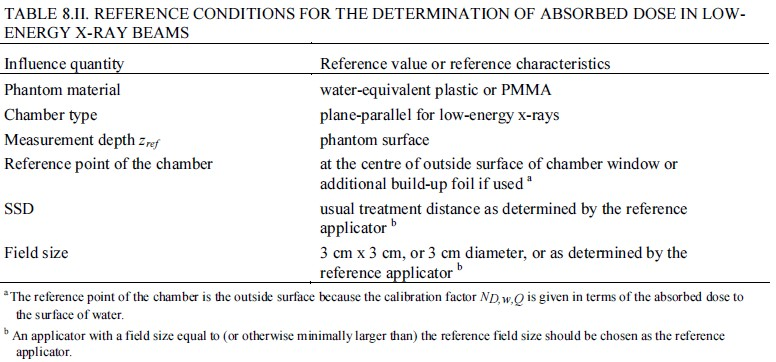
\includegraphics[width=0.8\textwidth]{Imagens/condicoesReferenciaDosekv.jpg}
		}%
		\caption{Condições de referência para determinação da dose absorvida para feixes de baixo kV}
		\label{fig:condicoesReferenciaDosekv}
	\end{figure}

	\begin{figure}[h]
		\centering
		\fcolorbox{DarkTurquoise}{white}{%
			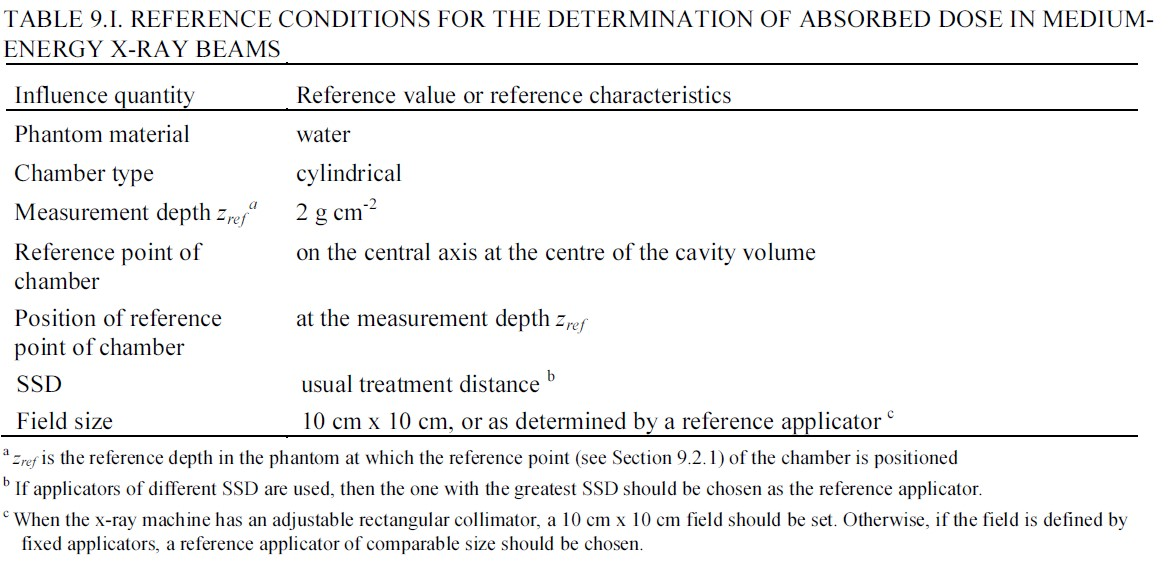
\includegraphics[width=0.8\textwidth]{Imagens/condicoesReferenciaDoseMediokv.jpg}
		}%
		\caption{Condições de referência para determinação da dose absorvida para feixes de médio kV}
		\label{fig:condicoesReferenciaDoseMediokv}
	\end{figure}

\section{Dosimetria de Fontes de Braquiterapia}

	As fontes de braquiterapia são geralmente calibradas usando \textcolor{MediumOrchid}{\textbf{\textit{uma câmara de poço com cavidade de ar}}}. O \textcolor{MediumOrchid}{\textbf{\textit{TG-43}}}, ``\textbf{\textit{Dosimetry of Intersticial Brachytherapy Sources}}'' e seus updates posteriores descrevem um método geral para calcular a \textcolor{MediumOrchid}{\textbf{\textit{dose absorvida}}} em qualquer ponto a partir de um valor de \textcolor{MediumOrchid}{\textbf{\textit{força kerma no ar}}}, $S_k$, dada em  unidades de $\mu Gy \cdot m^2 \cdot h^{-1}$, que recebe o símbolo U. A câmara do poço é calibrada em termos dessa força de kerma no ar, obtendo um fator de calibração, fornecido por um laboratório credenciado, para converter a leitura atual da câmara poço em força kerma no ar (também chamada de intensidade kerma no ar).

	A câmara do poço \textcolor{MediumOrchid}{\textbf{\textit{pode ser aberta para o ar ou pressurizada}}} para \textcolor{MediumOrchid}{\textbf{\textit{aumentar o sinal}}} da câmara. Caso seja utilizado uma câmara de poço pressurizada, é importante realizar \textcolor{MediumOrchid}{\textbf{\textit{medidas de constância da pressão interna}}} para garantir que não houve vazamento na câmara. 
	
	A \textcolor{MediumOrchid}{\textbf{\textit{resposta}}} da câmara poço depende da \textcolor{MediumOrchid}{\textbf{\textit{posição da fonte dentro da cavidade}}} formada pelo poço. Um \textcolor{MediumOrchid}{\textbf{\textit{suporte de fonte}}} (holder) é usado para \textcolor{MediumOrchid}{\textbf{\textit{posicionar}}} de forma reprodutiva a fonte no \textcolor{MediumOrchid}{\textbf{\textit{centro do cavidade}}}. O holder varia para fontes LDR e HDR e \textcolor{MediumOrchid}{\textbf{\textit{deve ser enviado junto com a câmara de poço para calibração}}} para que as condições exatas possam ser repetidas nab rotina clínica.

	
	Para sementes de \textcolor{MediumOrchid}{\textbf{\textit{baixa taxa de dose (LDR)}}}, a fonte é simplesmente colocada no suporte, que é \textcolor{MediumOrchid}{\textbf{\textit{projetado para posicionar a semente na área de resposta uniforme}}}. Porém, se possível, é ideal que exista uma indicação visual de que a semente está na posição correta para garantir a reprodutibilidade das medidas.

	Para sistemas de \textcolor{MediumOrchid}{\textbf{\textit{afterloader remoto}}} utilizados em braquiterapia de \textcolor{MediumOrchid}{\textbf{\textit{alta taxa de dose (HDR)}}}, a fonte geralmente é escalonada (realizada leituras no crescimento da escala) ao longo do comprimento da cavidade da câmara poço, inserindo um cateter fino conectado à unidade HDR no suporte para \textcolor{MediumOrchid}{\textbf{\textit{encontrar a posição de leitura máxima}}}, também chamado de ponto ideal \textcolor{MediumOrchid}{\textbf{\textit{(``sweet spot'')}}}. Esta posição deve ser consistente de medição para medição, mas o processo de escalonamento garante que a leitura correta seja obtida.

	Para \textcolor{MediumOrchid}{\textbf{\textit{fontes de baixa energia}}} como \ce{^{125}I} ou \ce{^{103}Pd}, a calibração deve ser obtida para o \textcolor{MediumOrchid}{\textbf{\textit{modelo específico}}} de semente utilizada clinicamente. Isso se deve ao fato de que \textcolor{MediumOrchid}{\textbf{\textit{o espectro de energia é muito afetado pela construção da semente}}}. Para fontes de energia mais altas, como \ce{^{192}Ir}, um \textcolor{MediumOrchid}{\textbf{\textit{valor genérico}}} pode ser usado.

	O protocolo do IPEM (``\textit{Institute of Physics and Engineering in Medicine}'') para fontes de \ce{^{192}Ir} utiliza a \textcolor{MediumOrchid}{\textbf{\textit{taxa de referência de kerma no ar (RAKR)}}}, dada em $Gy \cdot s^{-1}$ a 1 m. É então fornecido um \textcolor{MediumOrchid}{\textbf{\textit{coeficiente de conversão}}} para força kerma no ar para que os resultados possam ser comparados com o formalismo do TG-43.

	Ao calibrar uma fonte de \ce{^{192}Ir}, a câmara do poço deve estar a \textcolor{MediumOrchid}{\textbf{\textit{1 m}}} de qualquer \textcolor{MediumOrchid}{\textbf{\textit{parede}}} ou \textcolor{MediumOrchid}{\textbf{\textit{material espalhador}}} e deve ser colocada em um \textcolor{MediumOrchid}{\textbf{\textit{aparato de plástico}}}. A câmara do poço deve ser deixada na sala por tempo suficiente para permitir o \textcolor{MediumOrchid}{\textbf{\textit{equilíbrio térmico}}}, que pode ser de até 7 horas para uma diferença de temperatura de 4 °C usando uma câmara do poço Standard Imaging HDR 1000 Plus. \textcolor{MediumOrchid}{\textbf{\textit{Devem ser aplicadas correções de densidade do ar, recombinação iônica e do eletrômetro}}}. 

	\begin{wrapfigure}{r}{0.5\textwidth}
		\centering
		\fcolorbox{DarkTurquoise}{white}{%
			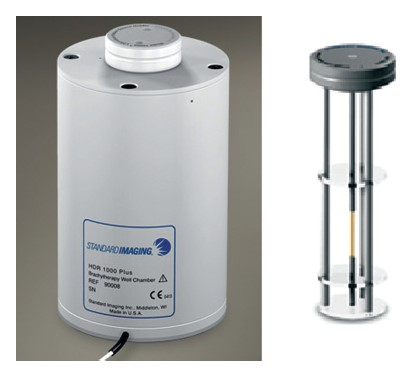
\includegraphics[width=0.45\textwidth]{Imagens/camaraPoco.jpg}
		}%
		\caption{Câmara Poço}
		\label{fig:camaraPoco}
	\end{wrapfigure}

	Outro documento utilizado é o \textcolor{MediumOrchid}{\textbf{\textit{TG-56}}}, ``\textbf{\textit{Code of Practice for Brachytherapy Physics}}''. Ambos documentos recomendam a utilização de um \textcolor{MediumOrchid}{\textbf{\textit{sistema terciário}}} para confirmar a \textcolor{MediumOrchid}{\textbf{\textit{constância do sistema secundário}}} utilizado na calibração, podendo ser \textcolor{MediumOrchid}{\textbf{\textit{outra câmara poço}}} ou uma \textcolor{MediumOrchid}{\textbf{\textit{câmara do tipo farmer}}} colocada em um ``jig'' (template, suporte fixo\dots) a \textcolor{MediumOrchid}{\textbf{\textit{10 cm}}} de distância da fonte.

	Quanto à \textcolor{MediumOrchid}{\textbf{\textit{calibração de sementes esterilizadas}}} para implantes intersticiais, o TG-56 recomenda que pelo menos \textcolor{MediumOrchid}{\textbf{\textit{10\% do lote ou 10 fontes, o que for maior, devem ser analisadas pelo físico local para sementes soltas}}}. Para \textcolor{MediumOrchid}{\textbf{\textit{fontes em fitas ou fios (stranded)}}}, a recomendação é de \textcolor{MediumOrchid}{\textbf{\textit{5\% ou 5 fontes, o que for menor}}}. Para atender a esse requisito, \textcolor{MediumOrchid}{\textbf{\textit{fontes extras}}} do mesmo lote podem ser solicitadas para fins de calibração, o que aumentará o custo. Alternativamente, as sementes de calibração podem ser encomendadas \textcolor{MediumOrchid}{\textbf{\textit{não estéreis}}} e então \textcolor{MediumOrchid}{\textbf{\textit{testadas}}} no local e \textcolor{MediumOrchid}{\textbf{\textit{re-esterilizadas}}}.

	Ao calibrar uma fonte de braquiterapia, é feita uma \textcolor{MediumOrchid}{\textbf{\textit{comparação}}} com o \textcolor{MediumOrchid}{\textbf{\textit{certificado de calibração emitido pelo fabricante da fonte}}}. O TG-56 recomenda que os valores devem estar acordados dentro de \textcolor{MediumOrchid}{\textbf{\textit{3\%}}}. Desvios entre \textcolor{MediumOrchid}{\textbf{\textit{3\%}}} e \textcolor{MediumOrchid}{\textbf{\textit{5\%}}} devem ser \textcolor{MediumOrchid}{\textbf{\textit{investigados}}} de modo que um sistema de dosimetria terciário ajudará nesta investigação. \textcolor{MediumOrchid}{\textbf{\textit{Diferenças superiores a 5\%}}} devem ser informadas ao fabricante. Se a fonte fizer parte de um lote a ser usado na implantação de sementes, a média do lote deve estar de acordo com a calibração do fabricante em 3\% e todas as fontes devem estar dentro de 5\% da média.

\section{Dosimetria em Feixes de Prótons}

	O TRS-398 descreve a determinação da dose absorvida em feixes de prótons. As \textcolor{MediumOrchid}{\textbf{\textit{câmaras de placas paralelas}}} podem ser usadas para \textcolor{MediumOrchid}{\textbf{\textit{todas as energias de feixe}}}, mas as \textcolor{MediumOrchid}{\textbf{\textit{câmaras cilíndricas}}} podem ser usadas \textcolor{MediumOrchid}{\textbf{\textit{apenas}}} para qualidades de feixe na profundidade de referência \textcolor{MediumOrchid}{\textbf{\textit{$R_{res}$ $>$ 0.5 g $cm^{-2}$}}}. As câmaras cilíndricas são preferíveis quando apropriado. 
	
	$R_{res}$ é o \textcolor{MediumOrchid}{\textbf{\textit{intervalo residual}}} e é definido como a \textcolor{MediumOrchid}{\textbf{\textit{distância do centro do pico de Bragg espalhado (SOBP) até os 10\% da profundidade distal}}}. \textcolor{MediumOrchid}{\textbf{\textit{$R_{res}$}}} é usado como o \textcolor{MediumOrchid}{\textbf{\textit{índice de qualidade do feixe}}} no protocolo e é determinado a partir de medidas de dose na profundidade feitas com uma câmara de placas paralelas. A \textcolor{MediumOrchid}{\textbf{\textit{ionização na profundidade}}} é convertida em \textcolor{MediumOrchid}{\textbf{\textit{dose na profundidade}}} aplicando \textcolor{MediumOrchid}{\textbf{\textit{razões do poder de freamento}}}. Portanto, deve ser aplicado os fatores de correção \textcolor{MediumOrchid}{\textbf{\textit{$K_{ion}$ e $K_{pol}$}}} na curva de ionização\textcolor{MediumOrchid}{\textbf{\textit{ caso esses fatores variem}}} com a profundidade.

	O \textcolor{MediumOrchid}{\textbf{\textit{ponto de referência}}} para a medida da dose absorvida é definido no \textcolor{MediumOrchid}{\textbf{\textit{centro do SOBP}}}. Um dos fatores que afeta a precisão da posição do ponto de referência é a \textcolor{MediumOrchid}{\textbf{\textit{ondulação no SOBP}}}, que deve ser \textcolor{MediumOrchid}{\textbf{\textit{$< \pm 3$\%}}}. O protocolo possui tabelas para os valores de \textcolor{MediumOrchid}{\textbf{\textit{$k_{Q,Q_0}$}}} que são todos valores calculados com \textcolor{MediumOrchid}{\textbf{\textit{$Q_0$ igual a \ce{^{60}Co}}}}. Correções de \textcolor{MediumOrchid}{\textbf{\textit{densidade do ar}}}, \textcolor{MediumOrchid}{\textbf{\textit{recombinação iônica}}} e \textcolor{MediumOrchid}{\textbf{\textit{polaridade}}} são usadas ao calcular a dose absorvida. Para \textcolor{MediumOrchid}{\textbf{\textit{campos pequenos}}}, com tamanho menor que duas vezes o diâmetro da cavidade de ar da câmara de placas paralelas, um dosímetro mais adequado, como um \textcolor{MediumOrchid}{\textbf{\textit{diodo}}} ou microcâmara, deve ser utilizado. Este detector deve ser \textcolor{MediumOrchid}{\textbf{\textit{calibrado por comparação}}} com a câmara de placas paralelas em um tamanho de campo maior.

\section{Incertezas Dosimétricas}

	A \ref{fig:incertezaDosimetricaExternalBeam} e a \ref{fig:incertezaCalibracaoKermaAr} apresentam os erros associados a dosimetria de referência em feixes de teleterapia e à calibração da força kerma ar, respectivamente. 

	Para feixes de \textcolor{MediumOrchid}{\textbf{\textit{teleterapia}}}, há uma incerteza geral de \textcolor{MediumOrchid}{\textbf{\textit{$\pm$ 1.5\%}}} enquanto que a incerteza propagada na determinação da \textcolor{MediumOrchid}{\textbf{\textit{força kerma ar}}} é de \textcolor{MediumOrchid}{\textbf{\textit{$\pm$ 2.6\%}}}.

\begin{figure}[h]
    \centering
    \fcolorbox{DarkTurquoise}{white}{%
        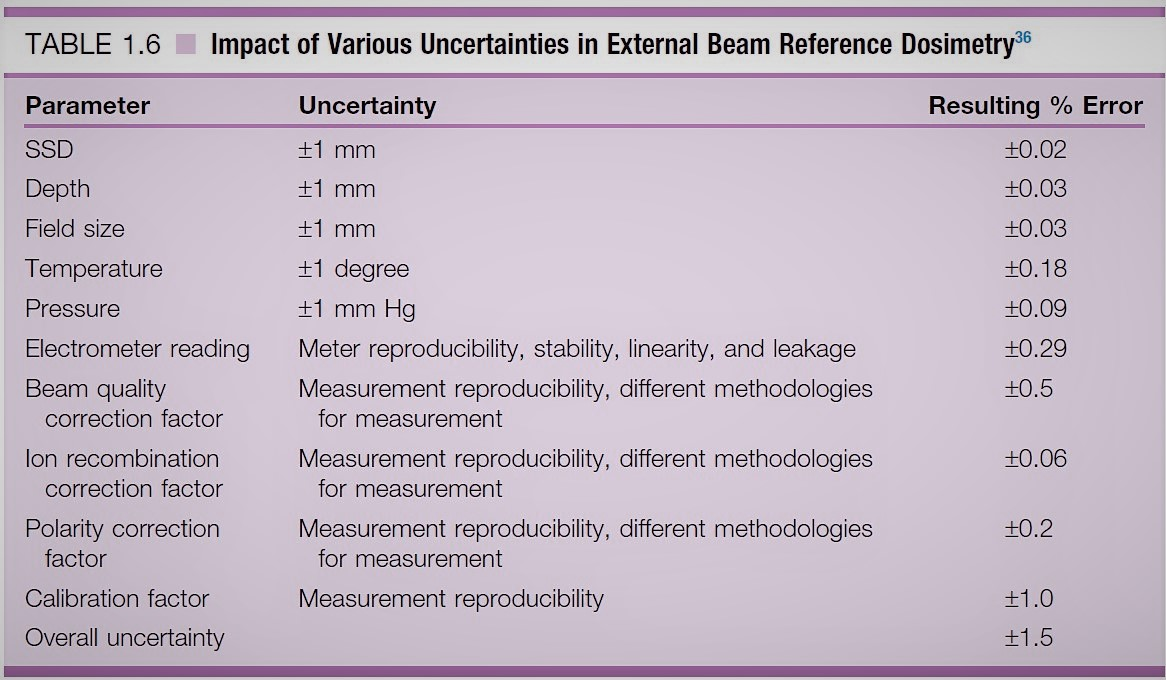
\includegraphics[width=0.8\textwidth]{Imagens/incertezaDosimetricaExternalBeam.jpg}
    }%
    \caption{Impacto das incertezas relacionadas a dosimetria de referência de feixes externos de radioterapia}
    \label{fig:incertezaDosimetricaExternalBeam}
\end{figure}

\begin{figure}[h]
    \centering
    \fcolorbox{DarkTurquoise}{white}{%
        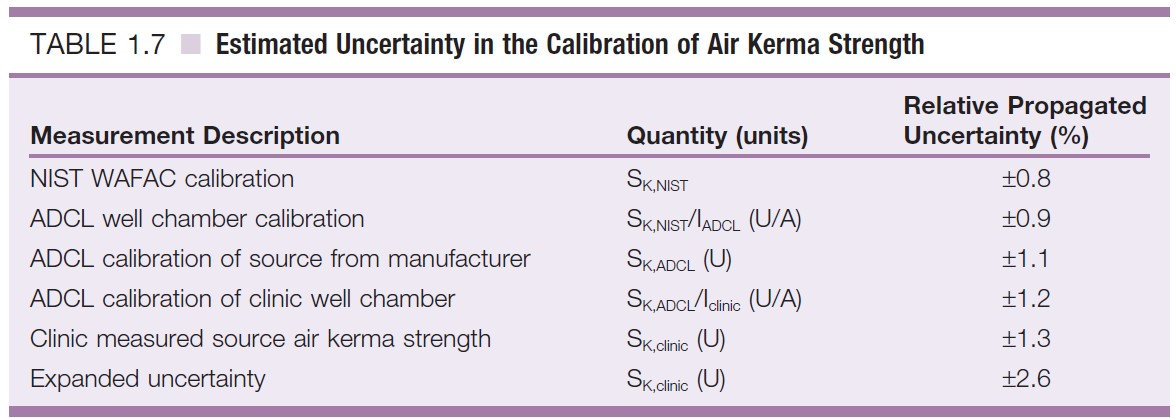
\includegraphics[width=0.8\textwidth]{Imagens/incertezaCalibracaoKermaAr.jpg}
    }%
    \caption{Estimativas de incertezas na calibração da força kerma no ar.}
	\label{fig:incertezaCalibracaoKermaAr}
\end{figure}


\bibliography{ref.bib}
\end{document}